\section{Problema 2}

\subsection{Introducción}

En este problema se debe determinar el área total de un campo que queda protegida de una plaga de langostas. Para considerar aislada una porción del mismo, ésta debe estar completamente encerrada por vallas de altura mayor o igual a la del salto de las langostas. A partir de entender esto, pensamos de qué manera podíamos modelar el campo, partirlo en "porciones" (que luego llamaríamos \textit{parcelas}), y recorrerlas chequeando si podíamos infestarlas de langostas. Realizando este recorrido, esperábamos lograr identificar el área infestada y contando con el área total, obtener mediante una simple resta el área protegida.\\
\indent Debido a cómo está presentado el problema, y los datos de entrada, consideramos el campo como el primer cuadrante de un sistema de ejes cartesianos. Así, el molino donde se ubica la Tía queda representado por el origen - $(0,0)$ - y cada valla se ubica en el plano con respecto a este punto. Además, a partir de la longitud y orientiacón de cada valla inferimos el extremo donde termina. De esta manera, al procesarlas todas, pudimos obtener cuáles eran las coordenadas máximas en sentido del eje de ordenadas y abscisas, con lo cual fijamos los límites del campo sumando uno a esos valores.\\
\indent En un primer momento nos propusimos modelar el campo utilizando esta información pero volcándola en una matriz donde cada posición de la misma se correspondiera con un sector del campo de lado $1x1$. Nuestra idea era posicionar las vallas en la matriz, determinando qué cuadrados quedaban bloqueados, y luego infestar de alguna manera pintando las posiciones de la matriz a las que sí podíamos acceder. Rápidamente desistimos de esta idea (a pesar de que luego la retomaríamos optimizando nuestras estructuras) dado que manejarnos con esa matriz no nos permitía cumplir con la cota de complejidad pedida. Las dimensiones de la matriz hubieran sido proporcionales a la superficie del campo, la cual a su vez quedaba determinada por la ubicación de una valla, variable sobre la cual no podíamos suponer nada y no se relacionaba con las magnitudes que necesitábamos contar.\\
\indent El segundo intento consistió en pensar cada valla como un nodo de un grafo, donde las aristas estuvieran representadas por las intersecciones entre las vallas. Luego, los vecinos de un nodo/valla serían otros nodos/vallas con los que se tocara en cualquier punto. Viéndolo así, buscamos interpretar las porciones completamente valladas como los ciclos de ese grafo. Una vez que tuvieramos identificados los ciclos, debíamos ver cuáles eran válidos, cuáles incluían a otros, y así procesar demasiados casos particulares. No pudimos llegar a esa instancia, pues antes nos encontramos con la dificultad de contar e identificar ciclos. Sin embargo, al pensar en cómo podíamos clasificar los ciclos, introdujimos un detalle que luego perduraría en nuestra solución final: a medida que procesamos cada valla para alojarla en nuestra estructura dejamos de lado aquella cuya altura sea menor a la que saltan las langostas. Así nos aseguramos que en el resto del problema vamos a mirar vallas que sean candidatas a proteger una porción del campo, con lo cual prescindimos de realizar este chequeo y mirar vallas innecesariamente.\\
\indent Frente a un panorama incierto, y habiendo descartado dos intentos de solución, logramos desarrollar una tercera idea que terminaría siendo correcta para la resolución del problema tanto en términos de la solución esperada como de la complejidad temporal. 

\subsection{Representación del Problema}

El primer boceto de solución con que contamos intentaba trazar una cuadrícula sobre el campo y luego implementar eso sobre una matriz. Esto nos obligaba a movernos de a un paso a medida que infestabamos el terreno, transformando nuestra complejidad en algo que no se relacionaba con la cantidad de vallas, y que seguramente fuera muy superior a este número. Ahora bien, considerando este movimiento, concebimos que no tenía sentido pensar que la plaga de langostas se moviera en una dirección dada de a pasos tan pequeños ya que en última instancia podría moverse hasta que se topara con una valla, infestando en un solo paso grande varios de nuestros pequeños sectores anteriores.\\
\indent Dividimos entonces la representación del campo en distintas etapas de procesamiento (ver \textbf{Fig. ~\ref{fig:ej2Mapeo} }). Primero, extendimos las vallas iniciales en megavallas que atravesaran el terreno del campo de un extremo a otro. Para esto contamos con dos diccionarios de megavallas, uno correspondiente a las verticales y otro a las horizontales. Cada definición se hace en base a una clave (entero) que representa la coordenada vertical u horizontal en que se extiende esa megavalla, y un significado que no es otra cosa que una lista de las vallas originales que viven en ese segmento y cuya altura impide el salto de las langostas. Además, la manera en que representamos las vallas es a través de un par de coordenadas, cuyas componentes $x$ e $y$ indican el comienzo y fin de la valla respectivamente.

\clearpage

\begin{figure}[h]
\centering                                                       
        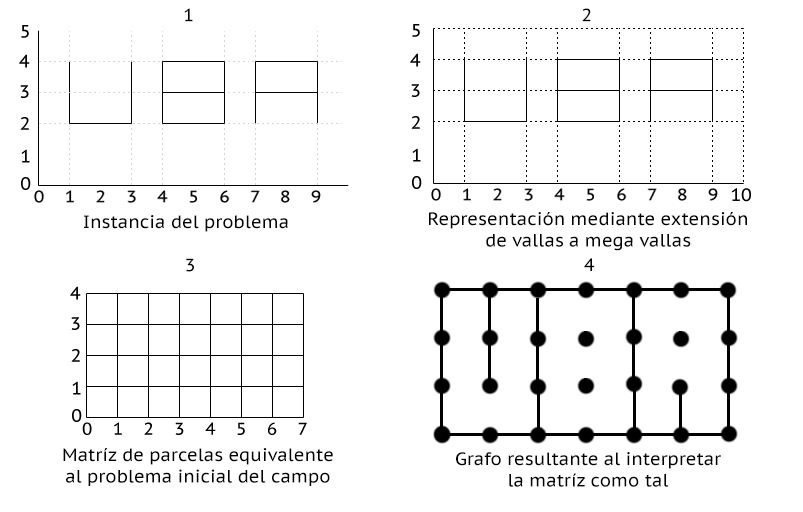
\includegraphics[width=320pt]{./figs/mapeoParcelas.png}
	\caption{Transformación del Problema Inicial}
	\label{fig:ej2Mapeo}
\end{figure}

Como se puede observar en la segunda imagen de la Fig. anterior, las intersecciones de las megavallas definen una cuadrícula de parcelas cuyo tamaño es variable y heterogéneo. Sin embargo, todas tienen forma rectangular, y a partir de la información almacenada hasta el momento es posible determinar su área y si el acceso a las parcelas contiguas está impedido o no por algún tramo de valla. Esto nos permitió armar una matriz que representara esta cuadrícula de dimensiones $\#megavallasHor*\#megavallasVer$, y cuyas posiciones alojaran un objeto parcela que contuviera la información antes mencionada, además de agregar un atributo booleano para determinar si la parcela era infestable (necesario para recorrer la matriz con una adaptación de 'BFS'). Este procesamiento se realiza a través de la función $armarParcelas$ (ver \textsl{Pseudocódigo 2}). Para lograr el correcto armado y mapeo del campo a esta matriz necesitamos contar con las megavallas ordenadas en forma ascendente (garantizado por el diccionario) así como también las vallas contenidas en cada una. En un principio, implementamos cada megavalla como otro diccionario que tuviera como clave el comienzo de una valla y como significado su fin. Esto nos garantizaba el orden necesario para recorrerlas, pero nos imponía un costo logarítmico para acceder a su significado. Dado que esto nos arruinaba la complejidad, acudimos a la implementación de la colección de vallas mediante una lista de manera tal que, al terminar de procesar todas las vallas, ordenáramos cada colección y así pudieramos acceder a toda su información en tiempo constante. Por eso, en la resolución del problema, hay un llamado al método de Campo $ordenarVallas$ antes de armar la matriz de parcelas, pues en otro caso el algoritmo no sería correcto.\\
\indent Esta matriz de parcelas se corresponde con la etapa número 3 de la Figura ~\ref{fig:ej2Mapeo}. Como se explica en el análisis de complejidad, esta vez sí podemos pagar el costo de recorrer la matriz, ya que sus dimensiones se encuentran en función de la magnitud que nos interesa (\#vallas). Al interpretarla como un grafo, las posiciones (parcelas) pasaron a ser los nodos, mientras que las aristas entre un par de nodos implica que las langostas pueden moverse de esa parcela a su contigua (ver Fig. ~\ref{fig:ej2Mapeo}.4). Luego, todo el área que pudiera ser infestada por estos desalmados crustáceos representaría una componente conexa del grafo. Supusimos entonces que la plaga comenzaba a infestar el campo desde los bordes, con lo cual partiendo de la parcela origen aplicamos una adaptación de 'BFS' ($buscarArea$, \textsl{Pseudocódigo 3}) para infestar la componente conexa que contuviera los bordes. A través de este recorrido contamos el área que podía ser infestada, y luego se lo restamos al área total.

\clearpage


\subsection{Pseudocódigos}

\begin{algorithm}
\caption{armarParcelas (\textbf{in/out} campo: \textsl{Campo})}
\begin{algorithmic}[1]

\STATE $cantH \leftarrow$ cantidad de megavallas horizontales en el $campo$
\STATE $cantV \leftarrow$ cantidad de megavallas verticales en el $campo$
\STATE $cuadricula \leftarrow$ armar matriz de $cantH*cantV$
\WHILE{hay megavallas horizontales}
	\WHILE{hay megavallas verticales}
		\STATE crear una $parcela$ dada por las megavallas que la encierran
		\STATE definir en $parcela$ si se puede infestar en cada dirección
		\STATE definir en $parcela$ el área que comprende
		\STATE asignar $parcela$ a la posición correspondiente en $cuadricula$
	\ENDWHILE
\ENDWHILE
\STATE guardar $cuadricula$ en $campo$
\end{algorithmic}
\end{algorithm}

\begin{algorithm}
\caption{buscarArea (\textbf{in/out} campo: \textsl{Campo}) $\rightarrow$ res: \textsl{Integer}}
\begin{algorithmic}[1]

\STATE $cola \leftarrow$ crear cola de parcelas vacía
\STATE marcar $parcela$ $origen$ del campo como infestable
\STATE agregar $parcela$ $origen$ a la cola
\STATE $areaInfestada \leftarrow 0$

\WHILE{hay parcelas en la $cola$}
	\STATE $parcela \leftarrow$ pop primer elemento de la cola
	\STATE $areaInfestada \leftarrow areaInfestada$ $+$ área de $parcela$ 
	\STATE agregar parcelas contiguas a $parcela$ que se puedan infestar
\ENDWHILE
\RETURN área de $campo$ - $areaInfestada$
\end{algorithmic}
\end{algorithm}

\clearpage

